\documentclass[spanish]{beamer}

%%% CODIFICACIÓN

%\usepackage[x11names, rgb, html]{xcolor}
\usepackage[utf8]{inputenc}
\usepackage[spanish]{babel}
\usepackage{graphics,tikz}
\usepackage{algpseudocode}
\usepackage[plain]{algorithm}

%%% FUENTES

\usepackage[T1]{fontenc}
\usepackage[familydefault,regular]{Chivo}
\usepackage{newtxsf} % Fuente de matemáticas
\usepackage{mathastext}
\usepackage[scaled=.85]{FiraMono}

\setbeamertemplate{navigation symbols}{}

%%% COLORES 

\definecolor{50}{HTML}{FFEBEE}
\definecolor{100}{HTML}{FFCDD2}
\definecolor{200}{HTML}{EF9A9A}
\definecolor{300}{HTML}{E57373}
\definecolor{400}{HTML}{EF5350}
\definecolor{500}{HTML}{F44336}
\definecolor{600}{HTML}{E53935}
\definecolor{700}{HTML}{D32F2F}
\definecolor{800}{HTML}{C62828}
\definecolor{900}{HTML}{B71C1C}

%% Colores de Solarized

\definecolor{sbase03}{HTML}{002B36}
\definecolor{sbase02}{HTML}{073642}
\definecolor{sbase01}{HTML}{586E75}
\definecolor{sbase00}{HTML}{657B83}
\definecolor{sbase0}{HTML}{839496}
\definecolor{sbase1}{HTML}{93A1A1}
\definecolor{sbase2}{HTML}{EEE8D5}
\definecolor{sbase3}{HTML}{FDF6E3}
\definecolor{syellow}{HTML}{B58900}
\definecolor{sorange}{HTML}{CB4B16}
\definecolor{sred}{HTML}{DC322F}
\definecolor{smagenta}{HTML}{D33682}
\definecolor{sviolet}{HTML}{6C71C4}
\definecolor{sblue}{HTML}{268BD2}
\definecolor{scyan}{HTML}{2AA198}
\definecolor{sgreen}{HTML}{859900}

%% Colores del documento

\definecolor{background}{RGB}{237,237,237}
\definecolor{text}{RGB}{78,78,78}
\definecolor{accent}{RGB}{129, 26, 24}
\definecolor{accent2}{HTML}{814918}
\definecolor{accent3}{HTML}{136618}
\definecolor{accent4}{HTML}{0F4B4E}
\definecolor{accent5}{HTML}{681341}
\definecolor{accent6}{HTML}{1F1B5A}

%%% LISTINGS

\usepackage{listingsutf8}

%% Las tildes

\lstset{
  inputencoding=utf8/latin1
}

%% Colores de Solarized para listings

\lstset{
  % How/what to match
  % sensitive=true,
  language=C++,
  % Border (above and below)
  %frame=lines,
  % Line number
  numbers=left,
  % Extra margin on line (align with paragraph)
  xleftmargin=\parindent,
  % Put extra space under caption
  belowcaptionskip=1\baselineskip,
  % Colors
  % backgroundcolor=\color{sbase3},
  basicstyle=\scriptsize\ttfamily\color{text},
  keywordstyle=\color{900},
  commentstyle=\color{text},
  stringstyle=\color{700},
  numberstyle=\color{text},
  identifierstyle=\color{accent4},
  % Break long lines into multiple lines?
  breaklines=true,
  % Show a character for spaces?
  showstringspaces=false,
  tabsize=2,
  xleftmargin=1.5em,
}

\setbeamerfont{framesubtitle}{size=\normalfont\tiny}
\setbeamercolor{framesubtitle}{fg=white}


%%% AJUSTES DE BEAMER

% ¿Negrita en el título de diapositiva o no?
%\setbeamertemplate{frametitle}{\color{accent}\vspace*{1cm}\bfseries\insertframetitle\par\vskip-6pt}

\setbeamertemplate{frametitle}{\color{900}\vspace*{1cm}\insertframetitle\par\vskip-6pt}

\setbeamertemplate{itemize items}[circle] % Viñetas de itemize

%%% CONFIGURACIÓN DE COLORES DE BEAMER

\setbeamercolor{background canvas}{bg=background}
\setbeamercolor{normal text}{fg=text}
\setbeamercolor{alerted text}{fg=900}
\setbeamercolor{block title}{fg=900}
\setbeamercolor{alerted text}{fg=900}
\setbeamercolor{itemize item}{fg=900}
\setbeamercolor{enumerate item}{fg=900}
\setbeamercolor*{title}{fg=900}
\setbeamercolor{qed symbol}{fg=900}
\usebeamercolor[fg]{normal text}

%%% PGFPLOTSTABLE

\usepackage{pgfplotstable}


\pgfplotstableset{
columns/0/.style={
     column name={Elementos},
   },
columns/1/.style={
     column name={Tiempo en segundos},
   },
}


%%% LISTINGS

\renewcommand{\lstlistingname}{Código fuente}

%%% INFORMACIÓN DEL DOCUMENTO

\title{Algorítmica: práctica 3}
\subtitle{Encontrar un recubrimiento minimal de un grafo}
\author{Sofía Almeida Bruno\\ Antonio Coín Castro\\ María Victoria Granados Pozo\\ Miguel Lentisco Ballesteros\\ José María Martín Luque\\ \vspace{1em}Grupo 2}
\begin{document}


\maketitle

\begin{frame}{Objetivo}

	Encontrar un recubrimiento minimal del grafo no dirigido G = (V, E).
	Un conjunto U $\subseteq$ V es un recubrimiento de G si cada arista en E incide en, al menos, un vértice o nodo de U.

	La solución que proporcionamos es el conjunto de nodos que forman el recubrimiento junto con el coste (número de nodos).
\end{frame}

\begin{frame}{Ejemplo}
	\begin{figure}[H]
		\centering 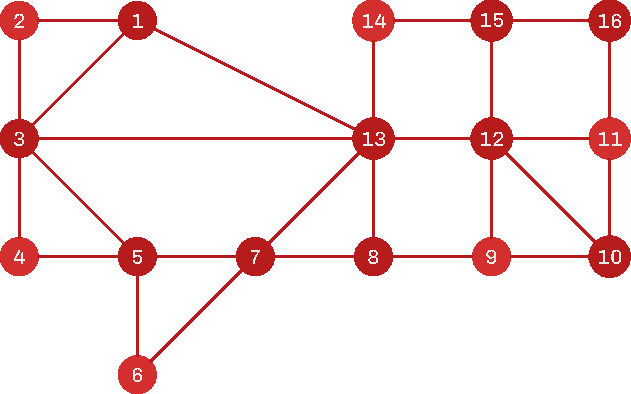
\includegraphics{./img/grafo-pres.pdf}
	\end{figure}
\end{frame}

\begin{frame}{Componentes Greedy}
	\begin{itemize}
		\item \textit{Lista de candidatos:} nodos del grafo
		\item \textit{Lista de candidatos utilizados:} nodos considerados
		\item \textit{Función solución:} no haya ninguna arista sin considerar
		\item \textit{Criterio de factibilidad:} el nodo no está en la lista de candidatos utilizados
		\item \textit{Función objetivo:} recubrimiento de coste mínimo
		\item \textit{Función de selección:} nodo en el que inciden más aristas
	\end{itemize}
\end{frame}

\begin{frame}
    \lstinputlisting[language=C++, linerange={12-25}, caption=Función de selección]{./../src/Algoritmo.cpp}
\end{frame}

\begin{frame}{Algoritmo}
	\lstinputlisting[language=C++, linerange={27-40}]{./../src/Algoritmo.cpp}
\end{frame}

\begin{frame}{Algoritmo}
	\lstinputlisting[language=C++, linerange={40-60}]{./../src/Algoritmo.cpp}
\end{frame}

\begin{frame}{Pseudocódigo}
$N \equiv$ número de nodos del grafo\\
$M \equiv$ número de nodos del recubrimiento\\
$L \equiv$ matriz de adyacencia\\
$T[1,\dots, M] \equiv$ vector de nodos del recubrimiento\\
$V[1,\dots, N] \equiv$ vector de incidencias
\end{frame}

\begin{frame}
\scalebox{0.68}{\begin{minipage}{1.45\linewidth}
\begin{algorithm}[H]
\begin{algorithmic}


\Function{RecubrimientoGrafoGreedy }{$L[1,\dots,N][1,\dots,N]\ $}
    \State $T = \emptyset$ \Comment Recubrimiento
    \For{$i=1,\dots,N$}
        \State $\displaystyle V[i] \gets \sum_{j=1}^N L[i][j]$ \Comment Número de incidencias del nodo $i$
    \EndFor

    \State $p \gets \text{Nodo con más incidencias} \left( V[p] \ge V[i] \ \ \forall i \right)$ \Comment Función de selección \\

    \While{$V[p] > 0$} \Comment Función solución

        \State $T \gets T \cup \{p\}$
        \State $V[p] \gets 0$
        \For{$j=1,\dots,N$}
            \If{Están conectados $p$ y $j$ \textbf{and} $V[j] > 0$ }
                \State $V[j] \gets V[j]-1$
            \EndIf
        \EndFor
        \State $p \gets \text{Nodo con más incidencias} \left( V[p] \ge V[i] \ \ \forall i \right)$ \Comment Función de selección

    \EndWhile \\
    \State \Return $T$
\EndFunction
\end{algorithmic}
\end{algorithm}

\end{minipage}}

\end{frame}

\begin{frame}{Ejemplo paso a paso}
	\begin{figure}[H]
		\centering 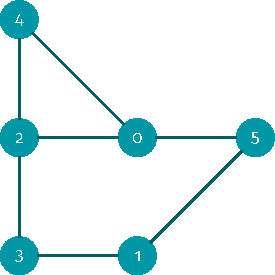
\includegraphics{./img/grafo-ejemplo-sin-recubrir-pres.pdf}
	\end{figure}

\end{frame}

%% FIXME Poner bien la presentación
\begin{frame}{Inicialización}
	N = num\_nodos = 6

	M = sol.coste = 0


	$\displaystyle  L = p.matriz\_adyacencia =
\begin{pmatrix}
  0 & 0 & 1 & 0 & 1 & 1 \\
  0 & 0 & 0 & 1 & 0 & 1 \\
  1 & 0 & 0 & 1 & 1 & 0 \\
  0 & 1 & 1 & 0 & 0 & 0 \\
  1 & 0 & 1 & 0 & 0 & 0 \\
  1 & 1 & 0 & 0 & 0 & 0
\end{pmatrix}$

	$\displaystyle  VI = incidencias =
\begin{pmatrix}
  3 \\
  2 \\
  3 \\
  2 \\
  2 \\
  2
\end{pmatrix} \hspace{2em} p = pos\_max = 0$

\end{frame}

\begin{frame}{Bucle while}
	incidencias[0] = 3 > 0\\
	T = \{0\}\\
	M = sol.coste = 1
	\begin{figure}[H]
		\centering 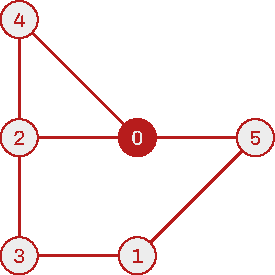
\includegraphics{./img/grafo-ejemplo-1-pres.pdf}
	\end{figure}
\end{frame}

\begin{frame}{}
	$\displaystyle  VI = incidencias =
	\begin{pmatrix}
	  3 \\
	  2 \\
	  3 \\
	  2 \\
	  2 \\
	  2
	\end{pmatrix} \implies  VI = incidencias =
	\begin{pmatrix}
	  0 \\
	  2 \\
	  2 \\
	  2 \\
	  1 \\
	  1
	\end{pmatrix}$

	\begin{figure}[H]
		\centering 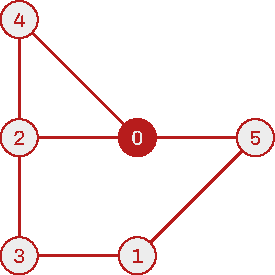
\includegraphics{./img/grafo-ejemplo-1-pres.pdf}
	\end{figure}
	p = pos\_max = 1

\end{frame}

\begin{frame}{Bucle while}
	incidencias[1] = 2 > 0\\
	T = \{0, 1\}\\
	M = sol.coste = 2
	\begin{figure}[H]
		\centering 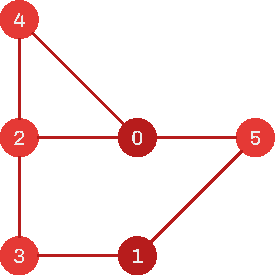
\includegraphics{./img/grafo-ejemplo-2-pres.pdf}
	\end{figure}
\end{frame}

\begin{frame}{}
	$$  VI = incidencias =
	\begin{pmatrix}
	  0 \\
	  2 \\
	  2 \\
	  2 \\
	  1 \\
	  1
	\end{pmatrix} \implies  VI = incidencias =
	\begin{pmatrix}
	  0 \\
	  0 \\
	  2 \\
	  1 \\
	  1 \\
	  0
	\end{pmatrix}$$
	\begin{figure}[H]
		\centering 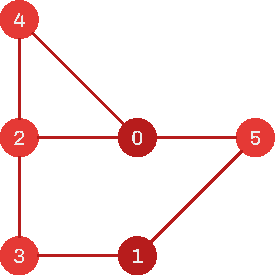
\includegraphics{./img/grafo-ejemplo-2-pres.pdf}
	\end{figure}
\end{frame}

\begin{frame}{Bucle while}
	incidencias[2] = 2 > 0\\
	T = \{0, 1, 2\}\\
	M = sol.coste = 3
	\begin{figure}[H]
		\centering 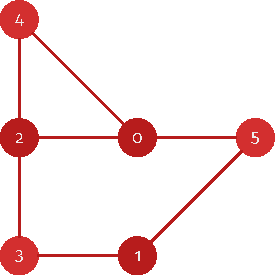
\includegraphics{./img/grafo-ejemplo-pres.pdf}
	\end{figure}
\end{frame}

\begin{frame}{}
	$$  VI = incidencias =
	\begin{pmatrix}
	  0 \\
	  0 \\
	  2 \\
	  1 \\
	  1 \\
	  0
	\end{pmatrix} \implies  VI = incidencias =
	\begin{pmatrix}
	  0 \\
	  0 \\
	  0 \\
	  0 \\
	  0 \\
	  0
	\end{pmatrix}$$
	\begin{figure}[H]
		\centering 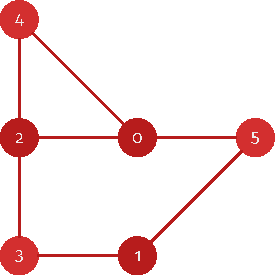
\includegraphics{./img/grafo-ejemplo-pres.pdf}
	\end{figure}
\end{frame}

\begin{frame}{Eficiencia teórica}
	Algoritmo de orden cuadrático: $O(|V|^2)$
	\lstinputlisting[language=C++, linerange={39-54}]{./../src/Algoritmo.cpp}

\end{frame}

\begin{frame}{Contraejemplo}

	\begin{figure}[H]
		\centering 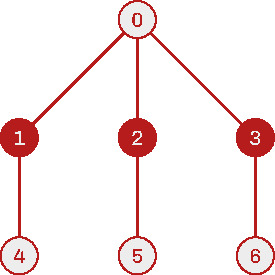
\includegraphics{./img/grafo2-pres.pdf}
	\end{figure}
\end{frame}

\begin{frame}{Contraejemplo}

	\begin{figure}[H]
		\centering 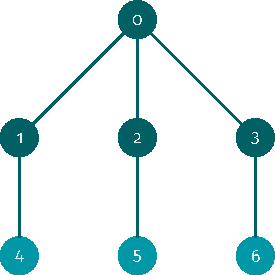
\includegraphics{./img/grafo2-no-minimal-pres.pdf}
	\end{figure}
\end{frame}

\begin{frame}{Ejemplo vida real}
	\begin{itemize}
		\item Hospitales y ciudades
		\item Red de comunicación
	\end{itemize}
\end{frame}

\end{document}
